
\documentclass[11pt, a4paper, german]{article}
\usepackage[utf8]{inputenc}
\usepackage{amsmath}
\usepackage{amsfonts}
\usepackage{amssymb}
\usepackage{algorithm}
\usepackage{algorithmic}
\usepackage{makeidx}
\usepackage{graphicx}
\usepackage{tabularx}
\usepackage{bbm}
\usepackage[ngerman]{babel}
\usepackage{BA_Titelseite}
\usepackage[colorlinks=false, pdfborder={0 0 0}]{hyperref}
\bibliographystyle{unsrt}

%Namen des Verfassers der Arbeit
\authornew{Boris Prochnau}

%Geburtsdatum des Verfassers
\geburtsdatum{22. Dezember 1989}
%Gebortsort des Verfassers
\geburtsort{Tartu}
%Datum der Abgabe der Arbeit
\date{\today}

%Name des Betreuers
% z.B.: Prof. Dr. Peter Koepke
\betreuer{Betreuer: Prof. Dr. Anton Bovier,\\ Dipl. Martina Baar und Dr. Loren Coquille}
%Name des Instituts an dem der Betreuer der Arbeit tätig ist.
%z.B.: Mathematisches Institut
\institut{Institut für Angewandte Mathematik}
%Titel der Bachelorarbeit
\title{Simulation normalisierter BPDL Prozesse und TSS Prozesse}
%Do not change!
\ausarbeitungstyp{Bachelorarbeit Mathematik}



\begin{document}

\maketitle
\tableofcontents



\clearpage
\section{Einleitung}
Ziel dieser Bachelorarbeit ist die Entwickelung eines Programms, das die Dynamik einer Population simulieren kann. Dar"uber hinaus wird die Erweiterung zu einem zweiten Programm vorgestellt welches besonders interessante Populationen, genannt "{}Trait Substitution Sequences"{}, simulieren kann.\\

Alle Simulationen basieren auf dem Modell, dass jedes Lebewesen einer Population (z.B. Pflanzen) ein bestimmtes Merkmal tr"agt. Bestimmt wird ein Merkmal durch Todesraten und einer Fortpflanzungsrate. Die Todesraten sind eine einfache nat"urliche Todesrate und eine durch Wettbewerb mit jedem anderem Individuum. Das hei"st diese Rate steigt mit der Anzahl der konkurrierenden Individuen.\\
Schlie"slich ist es jedoch die Entwicklung der Population und nicht der Individuen die simuliert werden soll. Deshalb kann man im simulierten Prozess zwar Tode und die Geburten verfolgen, aber nicht welches Individuum dieses Ereignis ausl"ost. Der "Ubergang zu dieser Sichtweise wird n"aher im 2. Kapitel beschrieben.\\

Das Programm sollte Parameter einlesen k"onnen und eine Oberfl"ache bieten auf die Simulation graphisch angezeigt wird. Tats"achlich wird das Programm mehr bieten und flexible Erweiterungsm"oglichkeiten beinhalten.\\
Die graphische Darstellung des Prozesses soll die M"oglichkeit bieten beobachten zu k"onnen ob sich ein Merkmal unter anderen Durchsetzten kann, es einen stabilen Zustand annimmt oder sicher dem Tod entgegen strebt.\\
\textit{N"aheres zum erwarteten Verhalten der Simulation fehlt noch}\\

Im letzten Teil werde ich noch kurz die Erweiterung auf TSS Prozesse vorstellen. Darin soll nicht nur das besonders interessante Verhalten vom Wechsel des dominanten Merkmals behandelt werden, sondern es wird eine verbesserte Laufzeit durch Interpolation vorgestellt die eine effiziente Simulation trotz sehr gro"ser Zeit und besonders pr"aziser Betrachtung von Aktionsreichen Gebieten anbietet.


%Dabei ist das Interesse besonders bei normalisierten BPDL Prozessen und schließlich auch bei TSS (trait subsitution sequence) Prozessen.\\
%Dabei reicht es nicht einfach eine Implementierung zu machen, denn durch die Zufallseigenschaft lässt sich nicht so einfach die Korrektheit verifizieren. Gerade bei TSS Prozessen ist die Anzahl der Mutationen und deren Abstände und Invasionschancen entscheidend.\\
%Zu diesem Zweck wird ein Teil der Arbeit diese Problemstellung behandeln.

\clearpage
\section{Modell}
Das verwendete Model wurde in \cite{Bolker_Spatial_moment,Bolker1997179,raey} eingef"uhrt. Dieses nutzt die drei grundlegenden Mechanismen von Darwins Evolutionslehre: Vererbung, Variation (Mutationen) und Selektion durch Wettbewerb um eine Menge von Merkmalen f"ur Individuen zu beschreiben. Diese bestimmen die F"ahigkeit des Individuums zu "uberleben und sich fortzupflanzen. Der daraus resultierende zeitstetige Sprung-Prozess wird BPDL Prozess (nach Bolker, Pacala, Dieckmann und Law) genannt.\\
Ziel wird es sein zwei spezielle BPDL-Grenzwert-Prozesse simulieren zu k"onnen.
	\subsection{Grundlagen}
	Sei $ X $ der Raum der Merkmale. Jedes Individuum hat genau ein solches Merkmal $ x \in X $. Der Einfachheit halber sei X eine Indexmenge: $ X = \{1,\dots, n\} $ repräsentativ für eine Durchzählung der Merkmale und im folgenden seien $ x,y \in X $ zwei solche Merkmale. Au"serdem gilt:
	\begin{itemize}
		\item Jedes Individuum kann sich asexuell fortpflanzen oder sterben.
		\item Fortpflanzungs- und Todeszeitpunkte k"onnen durch sogenannte exponentielle Uhren beschrieben werden (wie in \cite[S. 3]{fournier2004microscopic}). Diese Uhren haben exponentiell verteilte Weckzeiten. Durch die Gedächtnislosigkeit der Exponentialverteilung und wegen des Wettbewerbs, können und müssen alle Uhren nach dem ersten Klingeln neu gestellt werden. Durch den Einfluss des Wettbewerbs ist jede Todesrate abh"angig von der Anzahl an Konkurrenten die durch das zuerst eintretende Ereignis beeinflusst wird. 
		\item Die Fortpflanzung eines Individuums mit Merkmal $ x $ kann jedoch auch in der Geburt eines Individuums mit Merkmal $ y $ resultieren. Das wird durch die Mutationswahrscheinlichkeit kontrolliert.
	\end{itemize}
	Sp"ater wird deutlich dass die Zur"uckstellbarkeit der Uhren entscheiden ist um die Sichtweise von der Ebene des Individuums auf die der gesamten Population zu heben.\\
	Diese Todes und Fortpflanzungs- Ereignisse eines Individuums haben feste Raten die das dazugeh"orige Merkmal beschreiben.\\
	
	\begin{tabular}{r p{26em}}
		$ b(x) $: & Ist die Geburtenraten durch ein Individuum mit Merkmal $ x $.\\
		$ d(x) $: & Ist die natürliche Todesrate.\\
		$ c(x, y) $: & Ist die Todesrate durch Wettbewerb zwischen Individuen mit Merkmal x und y.\\
		$ \mu $: & Ist die Mutationswahrscheinlichkeit "{}auf die Nachbarn"{} mit je $ \frac{\mu}{2} $ pro Nachbar. \\
	\end{tabular}\\

	Schlie"slich lassen sich durch Superpositionsprinzip der Exponentialverteilung die beiden Todesraten zu einer gemeinsamen Todesrate zusammenfassen oder die arteigene Geburtenrate beschreiben.\\
	
	\begin{tabular}{ r p{18em} }
		$ b(x) \cdot (1 - \mu) $ & Ist die arteigene Geburtenrate eines Individuums mit Merkmal $ x $, also mutationsfreie Geburten.\\
		$ d(x) + \sum_{i=1}^{N_t} c(x, x_i) $ & Ist die gesamte Todesrate eines Individuums mit Merkmal x (mit $ N_t := $ \#Individuen zur Zeit t mit Merkmal $ x $ und $ x_i $ das Merkmal des i-ten Individuums).\\
		$ d(x) + \sum_{y=1}^{n} c(x,y) \cdot n_t(x) $ & Wie oben, nur mit $ n := $ \#Merkmale, und $ n_t(x) :=$ \#Individuen zur Zeit t mit Merkmal $ x $
	\end{tabular}\\

	Weil die Simulation die Entwicklung der Merkmale und nicht die Ereignisse der Individuen darstellt, ist es unpraktisch weiterhin die Raten jedes Individuums zu berechnen. Die letzte Darstellung der Todesrate ist z.B. praktischer f"ur die Betrachtung der Population durch den Fokus auf die Merkmale.  "Ahnlich k"onnen weitere Ereignisse zusammengefasst werden, so dass man z.B. eine Todesrate und eine arteigene Geburtenraten der Merkmale erstellen kann:
	
	\begin{itemize}
		\item Fortpflanzungsrate des Merkmals $ x $: 
		\[ B_1(x) = b(x) \cdot n_t(x) \]
		Oder alternativ die arteigene Geburtenrate (Wachstumsrate) des Merkmals $ x $: 
		\begin{align*}
			B_2(x)  & = (1 - \mu) \cdot b(x) \cdot n_t(x)\\
				  & + \frac{\mu}{2} \cdot b(x+1) \cdot n_t(x+1) \cdot \mathbbm{1}_{x<1}\\
				  & + \frac{\mu}{2} \cdot b(x-1) \cdot n_t(x-1) \cdot \mathbbm{1}_{x>1}
		\end{align*}
		\item Todesrate des Merkmals $ x $: 
		\[ D(x) = d(x) \cdot n_t(x) + n_t(x) \cdot \sum_{y=1}^{n} c(x,y) \cdot n_t(y) \]
	\end{itemize}
	Das entspricht 2 wesentlichen exponentiellen Uhren pro Merkmal. Eine für Tod und eine für Geburt innerhalb des Merkmals.\\
	\textit{F"ur die Simulation ist eine Gesamtrate für das Eintreten eines Ereignisses praktischer. Auf diese Weise wird nur auf das Eintreffen einer Uhr gewartet.}
	\begin{itemize}
		\item Ereignisrate des Merkmals $ x $ (Trait Rate):
		\[ TR(x) = B(x) + D(x) \]
		\item Totale Ereignis Rate (Total Event Rate): 
		\[ TER = \sum_{x \in X} TR(x)\]
	\end{itemize}
	Mit der Totalen Ereignisrate gibt es eine Rate die es erlaubt eine Zufallsvariable für das Eintreffen einer Variable zu ziehen. Anschließend ist es nur noch erforderlich (mit der Ziehung zwei weiterer Zufallsvairablen) festzustellen welchem Merkmal welches Ereignis zukommt. Das Zusammenfassen der Raten vereinfacht es dem Programm sp"atere Auswertungen und Funktionen bereitzustellen. So l"asst sich z.B. aus der Geburtenrate (Wachstumsrate) eines ausgestorbenen Merkmals die Mutationsrate ablesen, ohne weitere Berechnungen machen zu m"ussen.\\
	
	\subsection{BPDL Prozess}
	Die auf dem vorhergehenden Modell basierende Population wird durch die Zufallsvariable
	\[ \nu_t = \sum_{i=1}^{N_t} \delta_{x_i}, \quad x_i := \text{Das Merkmal des i-ten Individuums} \]
	beschrieben. Sie bildet Merkmale auf die Anzahl ihrer Repr"asentanten ab.\\
	Mit Zeitpfaden ist $ \nu_t $ ein stochastischer Prozess, genauer ein Markov Sprung Prozess auf dem Raum:
	\[ \nu_t \in M_F(X) = \left\{ \sum_{i=1}^{n} \delta_{x_i}, n \in \mathbb{N}, x_1, \dots, x_n \in X \right\} \]
	Man erkennt leicht die Sprungeigenschaft:
	\[ \int_X 1 \text{ } \nu_t(dx) = N_t 
	\text{ und }
	\int_X \mathbbm{1}_y(x) \text{ } \nu_t(dx) = n_t^{y} \]
	Normalerweise geh"ort zum Model des BPDL Prozesses, dass die Mutationen auf einem beliebigen Merkmal (nicht nur den Nachbarn) landen k"onnen und der Raum der Merkmale nicht unbedingt diskret sein muss. Eine Mutationswahrscheinlichkeit h"angt in diesem Fall vom Merkmal ab, also $ \mu(x) $. Und der Mutant hat dann Merkmal $ x + h $, wobei h eine zentrierte Zufallsvariable mit Dichte $ m(x,dh) $ auf $ (X - x) $ ist.
	F"ur einen solchen Prozess w"are der Generator definiert als:
	\begin{align*}
		L_{\phi(\nu)} &= \int_{X} b(x)(1-\mu)[\phi(\nu + \delta_x) - \phi(\nu)]\nu(dx)\\
					  &+ \int_{X}\int_{\mathbb{R}^d} b(x) \cdot \mu [\phi(\nu + \delta_{x+z}) - \phi(\nu)] m(x,dz) \nu(dx)\\
				  	  &+ \int_{X} d(x)[\phi(\nu - \delta_x) - \phi(\nu)]\nu(dx)\\
				 	  &+ \int_{X} \left( \int_{X} c(x,y) \nu(dy) \right) [\phi(\nu - \delta_x) - \phi(\nu)]\nu(dx)
	\end{align*}
	mit $ \phi: M_F \to \mathbb{R} $\\
	Mit unserem diskreten Raum X und der konstanten Mutationswahrscheinlichkeit zu Nachbarn vereinfacht sich der Generator. Der f"ur unser Model angepasster Generator hat somit folgende Form:
	\begin{align*}
		L_{\phi(\nu)} &= \sum_{i = 1}^{\infty} b(x_i)(1-\mu)[\phi(\nu + \delta_{x_i}) - \phi(\nu)] \cdot n(x_i)\\
		&+ \sum_{i \sim j} n(x_i) \cdot b(x_i) \cdot \mu \cdot 
		 [\phi(\nu + \delta_{x_j}) - \phi(\nu)] \cdot n(x_i)\\		 
		&+ \sum_{i = 1}^{\infty} (d(x) + \sum_{j = 1}^{\infty} c_{i,j} \cdot n(x_j))[\phi(\nu - \delta_x) - \phi(\nu)] \cdot n(x_i)\\
	\end{align*}
	mit $ \phi: M_F \to \mathbb{R} $ und $ n(x_i) := $ Anzahl Individuen mit Merkmal $ x_i $.\\	


\clearpage
\section{Eigenschaften des BPDL Prozesses\\ - anderer Name?}
In diesem Kapitel werden Eigenschaften des Prozesses n"aher untersucht die sp"ater oft bei der Simulation sichtbar sein sollen. Zun"achst wird dabei die Normalisierung eingef"uhrt die es auch einfacher macht Aussagen "uber das erwartete Verhalten des Prozesses bzw. der Population zu machen. 

\subsection{Normalisierung des BPDL Prozesses}
	Wie schon zuvor erwähnt ist es für uns wichtig die Tode und Geburten nicht auf der Ebene des Individuums, sondern der gesamten Population zu betrachten. Dazu wird die LPA(Large Population Approximation) Normalisierung aus \cite{fournier2004microscopic} eingeführt.\\
	Hierfür wird der Prozess mit einem Parameter K skaliert und es ergibt sich eine neue Zufallsvariable:
	\[ \nu_t^K := \frac{1}{K} \nu_t \]
	Um f"ur $ \nu_t^K $ das selbe Verhalten wie f"ur $ \nu_t $ zu erhalten, m"ussen einige Anpassungen vorgenommen werden.\\
	Zun"achst wird die Anfangsgröße $ n_0^K $ der Population proportional zu K gewählt.
	Die Raten für Geburten und natürliche Tode der Individuen bleiben unverändert. Da die Populationsgröße jedoch quadratisch in Wettbewerbsrate einfließt, sollte $ c^K = \frac{c}{K} $ gelten, da sonst die K-fach erh"ohte Population mit einem intensives Aussterben den Vergleich verf"alschen w"urde. \\
	Ein Beispiel f"ur eine LPA-Normalisierung sieht folgendermaßen aus:
	\begin{figure}[H]
		\centering
		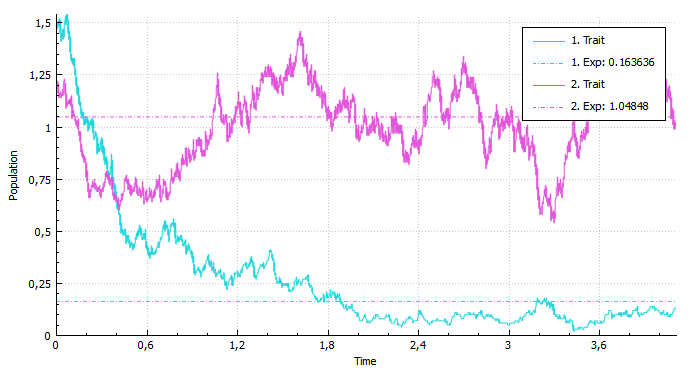
\includegraphics[width=0.7\linewidth]{./Pictures/LPANormalisierungK100}
		\caption[LPAK100]{LPA Normalisierung mit K=100}
		\label{LPA Normalisierung K=100}
	\end{figure}
	\begin{figure}[H]
		\centering
		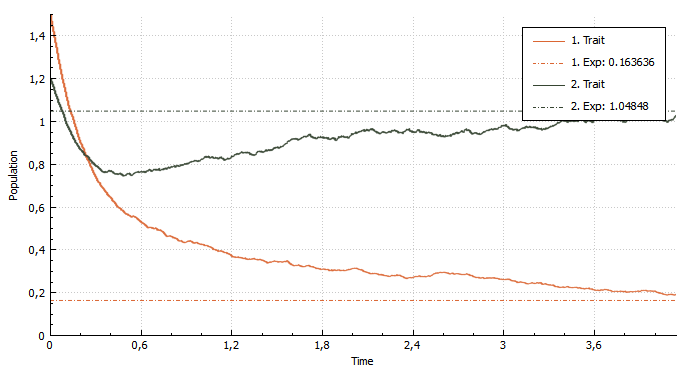
\includegraphics[width=0.7\linewidth]{./Pictures/LPANormalisierungK10000}
		\caption[LPAK100]{LPA Normalisierung mit K=10000}
		\label{LPA Normalisierung K=10000}
	\end{figure}
	\textit{Für eine Anfangspoulation die aus zwei Merkmalen bestehet, konvergiert der Prozess ohne Mutation gegen die Lösung der Konkurrenz Lotka-Volterra Gleichung für zwei Spezies (Siehe Kapitel 11 -Law of Large Numbers- von Ethien und Kurtz \cite{ethier2009markov}).}
	
	\subsection{Monomorphes Gleichgewicht}
	Wir stellen fest dass im Falle der monomorphen Population f"ur $ K \to \infty $, $ \nu_t $ gegen eine Funktion konvergiert die folgende Gleichung erf"ullt:
	\begin{align}
	\begin{split}
		\dot{n} &= (b(x) - d(x) - n \cdot c(x,x)) \cdot n \\
		n(0) &= n_0
	\end{split}
	\end{align}
	Wir wollen hieraus eine einen stabilen Zustand f"ur die Population ermitteln indem sich die Populationsgr"o"se nicht mehr "andern darf:
	\begin{align}
	\begin{split}
		0 &= \dot{n} = (b(x) - d(x) - nc(x,x))n\\
		\Rightarrow 0 &= b(x) - d(x) - nc(x,x)\\
		\Rightarrow \bar{n} &= \frac{b(x) - d(x)}{c(x,x)}
	\end{split}
	\end{align}
	$ \bar{n} $ ist somit das Gleichgewicht einer monomorphen Population. Zudem gilt dass stets eine Konvergenz der Population gegen $ \bar{n} $ f"ur beliebige Startwerte vorliegt.
	
%	Mit wachsendem K konvergiert das System gegen eine deterministische Funktion wie ich hieran noch erkl"aren muss \cite{ethier2009markov}.
	
	\subsection{Der TSS Grenzwertprozess}
	\textit{Die zuvor erw"ahnte Konvergenz  gilt auch f"ur d Merkmale mit Mutation mit dem selben Argument, da die Mutationen nach rechts und links begrenzt sind. Dadurch hat man immer nur maximal d Subpopulationen.\\
	Die Differenzialgleichung zu diesem Prozess konvergiert d-dimensional und "ahnelt bis auf den Mutationsanteil der d-dimensionalen Konkurrenz Lotka-Volterra Gleichung.}\\
	Genau wie bei der LPA-Normalisierung ergeben sich TSS-Prozesse(Trait Substitution Sequence) als Grenzprozesse von BPDL-Prozessen. Zu der LPA-Normalisierung sollten jedoch mit größer werdendem K die Mutationen seltener werden 
	\[ \left( \frac{1}{e^{VK}} << \mu_K << \frac{1}{K log(K)} \right), \] 
	also die Mutationswahrscheinlichkeit gegen 0 streben.\\ 
%	Warum $ \mu_K $ so gew"ahlt wird, ist n"aher im Kapitel "{}TSS Prozesse"{} erkl"art.\\ 
	\textbf{Frage:} Warum soll $ \mu_K $ in dem obigen Bereich gew"ahlt werden?\\
	\textbf{Antwort:} Dank Freidlin and Wenzell \cite{freidlin2012random} erwarten wir dass unsere dominante Spezies $ exp(cK) $ Zeiteinheiten im Gleichgewicht bleibt. Schlie"slich k"onnen wir so kontrollieren wie lange uns eine dominante Spezies die f"ur eine mutative Geburt in Frage kommt erhalten bleibt. Und dadurch dass die Mutationen exponentiell verteilt sind ben"otigt man ein eine Rate $ \mu_K >> \frac{1}{e^{cK}} $ um eine Zeit von $ exp(cK) $ nicht zu "uberschreiten, was die erste Schranke rechtfertigt.\\
	Um die zweite Schranke zu Rechtfertigen betrachten wir nun die Zeit die ein Mutant braucht um ein dominantes Merkmal aussterben zu lassen. Das wird uns die M"oglichkeit geben einer neuen Mutation so viel Zeit zu lassen bis das derzeit benachteiligte Merkmal ausgestorben ist.\\
	Angenommen es ereignet sich eine Mutation und der Mutant $ x $ ist fitter ($ f(x,y) > 0 $), so wird es mit positiver Wahrscheinlichkeit eine Invasion ausl"osen. Wenn man Branching Prozesse mit dem Lotka-Volterra System vergleicht, kommt man darauf dass die ben"otigte Zeit zum Verdr"angen und Aussterben des urspr"unglich dominanten Merkmals von der Ordnung $ \log(K) $ ist.
	Diese Invasion wird eine Zeit von der Ordnung $ \log(K) $ ben"otigen. Das l"asst sich folgern indem man Branching Prozesse mit 
	
	Skaliert man nun noch zusätzlich die Zeit, so führt dies dazu, dass der Prozess ausreichend Zeit zwischen zwei Mutationen hat um ein benachteiligtes Merkmal zu verdr"angen.
%	die Zeit, die ein Merkmal benötigt, um sich gegenüber einem anderen durchzusetzen und dieses zu verdrängen, infinitesimal klein wird. 
	Somit erlaubt uns die LPA-Annahme von einer deterministischen Populationsdynamik zwischen zwei Mutationen auszugehen \cite{raey}.\\
%	Somit simulieren die TSS-Prozesse eine Population, die zu jedem Zeitpunkt monomorph ist und sich im entsprechenden Gleichgewicht befindet.
	\begin{figure}[H]
		\centering
		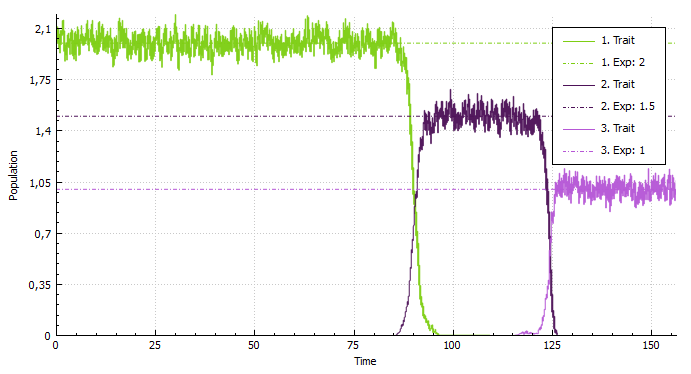
\includegraphics[width=1 \linewidth]{../BachelorArbeit/Pictures/TSS2_pure_small}
		\caption[TSS Prozess wechselnder Dominanz]{TSS Prozess mit: K = 1000 und $ 4 \cdot 10^6 $ Spr"ungen}
		\label{fig:TSS2_pure_small}
	\end{figure}
	
	\subsection{Die Fitnessfunktion}
	Spätestens jetzt wird die Fitnessfunktion interessant:
	\[ f(x,y) = b(x) - d(x) - c(x,y)\bar{n}_y \]
	Die Fitness-Funktion gibt an wie gut sich ein Mutant eines ausgestorbenen Merkmals in einem Gleichgewichtssystem durchsetzten kann. \\
	Man erkennt dass die Fitnessfunktion die Geburtenrate eines Mutanten $ b(x) $ dem zu erwarteten Widerstand, in Form der Todesrate $ - d(x) - c(x,y)\bar{n}_y $, gegen"uberstellt. Hierbei wird $ c(x,x) $ nicht ber"ucksichtigt weil es im Grenzwert mit K immer geringeren Einfluss hat, und gleicherma"sen haben wenige $ x  $ kaum Einfluss auf den Gleichgewichtszustand $ \bar{n}_y $ von $ y $. Damit begr"undet sich der Widerstand gegen den Mutanten durch die eigene Todesrate und die Konkurrenz der nahezu konstanten $ c(x,y)\bar{n}_y $. \\
	Die Fitness-Funktion ist also die asymptotische Wachstumsrate von x, wenn y sich in einem Gleichgewichtszustand befindet und nur wenige Individuen von Typ x in der Population vorhanden sind.\\
	Man kann in dieser Stelle bereits erahnen dass die Fitnessfunktion bzw. die Wachstumsrate eines Mutanten die M"oglichkeit bietet aussagen "uber die Invasionswahrscheinlichkeit bietet. Und tats"achlich wird in \cite{Champagnat20061127} eine Konvergenz f"ur $ K \to \infty $ von einer Konvergenz gegen 
	\[ \frac{\left[ f(y,x)\right]_+ }{b(y)} \]
	gesprochen. Begr"undet wird das durch [...]\\
	
	\subsection{Gleichgewicht im dimorphen Fall}
	Wir wissen mittlerweile dass die Population für $ K \to \infty $ gegen eine deterministische Funktion konvergiert. Angenommen es gibt wieder keine Mutation, dann gilt:\\
	\begin{align}
	\begin{split}
		\dot{n}_x & = n_x (b(x) - d(x) - c(x,x)n_x - c(x,y) n_y) \quad n_x(0) = n_{x,0} \\
		\dot{n}_y & = n_y (b(x) - d(x) - c(x,x)n_x - c(x,y) n_y) \quad n_x(0) = n_{x,0}
	\end{split}
	\end{align}
	Hier sieht man bereits leicht dass $ (\bar{n}_x, 0) $, $ (0, \bar{n}_y) $ und $ (0,0) $ stabile Zust"ande sind. Jedoch gibt es in diesem Fall auch einen Zustand indem eine Koexistenz beider Merkmale herrschen kann:
	\begin{align}
	\begin{split}
		n_x &= \frac{(b(x) - d(x))c(y,y)-(b(y)-d(y))c(x,y)}{c(y,y)c(x,x) - c(y,x)c(x,y)}\\
		n_y &= \frac{(b(y) - d(y))c(x,x)-(b(x)-d(x))c(y,x)}{c(y,y)c(x,x) - c(y,x)c(x,y)}
	\end{split}
	\end{align}
	Die BPDL Simulationen erkennen dimorphe und monomorphe Populationen und stellen stets einen passenden stabilen Zustand $ n_x $, bzw. $ \bar{n}_x $ dar. \\
	Um im dimorphen Fall zu entscheiden unter welchen Voraussetzungen zu welchem Gleichgewicht konvergiert wird, ben"otigen wir \cite[Proposition 3]{Champagnat20061127}. Darin werden die Gleichgewichte $ (\bar{n}_x, 0) $ und $ (0, \bar{n}_y) $ untersucht:
	\begin{itemize}
		\item[] Falls $ f(y,x) < 0 $, so ist $ (\bar{n}_x, 0) $ ist ein stabiler Zustand.
		\item[] Falls jedoch $ f(y,x) > 0 $ und $ f(x,y) < 0 $, so ist $ (0, \bar{n}_y) $ stabil und $ (\bar{n}_x, 0) $ ist instabil. In diesem Fall
	\end{itemize}
	Die Idee des Beweises ist [...]

\clearpage
	\noindent\rule{\textwidth}{2pt}
	\begin{center}
		$ <<< \quad \downarrow $ In Arbeit $ \downarrow \quad >>> $
	\end{center}
\section{Algorithmus zur Simulation eines normalisierten BPDL Prozesses}
	\subsection{Implementierung}
	Der Simulation liegt ein Algorithmus zugrunde der einen Sprung des Markov Sprung Prozesses durchführt. Im Code wird dazu die "{}EvolutionStep()"{} Funktion aufgerufen. (Es gibt auch Jump statt Step, aber mehrere Schritte)
	\begin{algorithm}[H]
		\caption{EvolutionStep()}
		\begin{algorithmic}[1]
			\ENSURE{A full evolution Step happened}
			\STATE calculateEventRates();
			\STATE sampleEventTime();
			\STATE changeATrait();
		\end{algorithmic}
	\end{algorithm}
	
	Von dieser werden folgende Berechnungen angestoßen:
		
	\begin{algorithm}[H]
		\caption{EvolutionStep()}
		\begin{algorithmic}[1]
			\ENSURE{A full evolution Step happened}
			\STATE ---$>$calculateEventRates();
			\STATE calculateTotalDeathRates()
			\STATE calculateTotalBirthRates()
			\STATE calculateTotalEventRate()
			\STATE ---$>$sampleEventTime();
			\STATE sampleEventTime();
			\STATE ---$>$changeATrait();
			\STATE choseTraitToChange();
			\STATE choseEventType();
			\STATE executeEventTypeOnTrait();
		\end{algorithmic}
	\end{algorithm}
	
	\subsection{Pseudocode}
	Schließlich der Ablauf der tatsächlichen Berechnung:
	
	\begin{algorithm}[H]
		\caption{EvolutionStep()}
		\begin{algorithmic}[1]
			\ENSURE{A full evolution Step happened}
			\REQUIRE $ t, X = \{0,\dots, n-1\} $
			\STATE ---$>$calculateEventRates();
			\FOR{ $ x \in X $ }
				\STATE $  D(x) := n_t(x) \cdot \left( d(x) + \sum_{y \in X} c(x,y) \cdot n_t(y) \right) $
				\STATE $ B(x) := \underbrace{b(x) \cdot (1 - \mu) \cdot n_t(x)}_{arteigene}  $
				\IF{$ x > 0 $}
					\STATE $ B(x) += \underbrace{b(x-1)\cdot n_t(x-1)}_{Mutation Links} \cdot \frac{\mu}{2} $
				\ENDIF
				\IF{$ x < n-1 $}
					\STATE $ B(x) += \underbrace{b(x+1)\cdot n_t(x+1)}_{Mutation Rechts} \cdot \frac{\mu}{2} $
				\ENDIF
				\STATE $ TotalTraitRate(x) = B(x) + D(x) $
			\ENDFOR
			\STATE $ TotalEventRate := \sum_{x \in X} TotalTraitRate(x) $
			
			\STATE ---$>$sampleEventTime();
			\STATE sample $ Z \sim exp(TotalEventRate) $
			\STATE $ t += Z $
			
			\STATE ---$>$choseTraitToChange();
			\STATE sample $ Y \sim U(0,TotalEventRate) $
			\FOR{$ x \in X $}
				\IF{$ Y \le TotalTraitRate(x) $}
					\STATE $ ChosenTrait := x $
					\STATE break
				\ENDIF
				\STATE $ Y -= TotalTraitRate(x) $
			\ENDFOR
			
			\STATE ---$>$choseEventType();
			\STATE sample $ Y \sim U(0,TotalTraitRate(ChosenTrait)) $
			\IF{$ Y \le B(ChosenTrait) $}
				\STATE isBirht := true
			\ELSE
				\STATE isBirth := false
			\ENDIF
			
			\STATE ---$>$executeEventTypeOnTrait();
			\IF{isBirth}
				\STATE $ n_t(ChosenTrait) += 1 $
			\ELSE
				\IF{$ n_t(ChosenTrait) \ge 0 $}
					\STATE $ n_t(ChosenTrait) -= 1 $
				\ENDIF
			\ENDIF
		\end{algorithmic}
	\end{algorithm}
	
	\subsection{Optimierung f"ur viele Merkmale}
	
\clearpage

\section{Das Programm}

Nun kommen wir zur eigentlichen Simulation. Damit ist sowohl die Darstellung als auch die Programmarchitektur gemeint. 
	\subsection{Aufgabenteilung und Flexibilität}
	Die Idee der getrennten Aufgabenbereiche geht darauf zurück dass eine möglichst große Unabhängigkeit zwischen Arbeitsschritten notwendig ist um das Programm flexibel zu halten und sogenannten "{}Coderot"{} - "{}faulen Code"{} zu verhindern. Das bedeutet dass das Programm mit steigender Komplexität zunehmend unflexibler wird, also das Hinzufügen weiterer Features oder das Ändern/Verbessern zu sogenanntem "{}undefiniertem Verhalten"{} führt. (kurze Erklärung zum Begriff).\\
	Die Architektur des Programms kann grob in drei Module gefasst werden. 
	\begin{figure}[H]
		\centering
		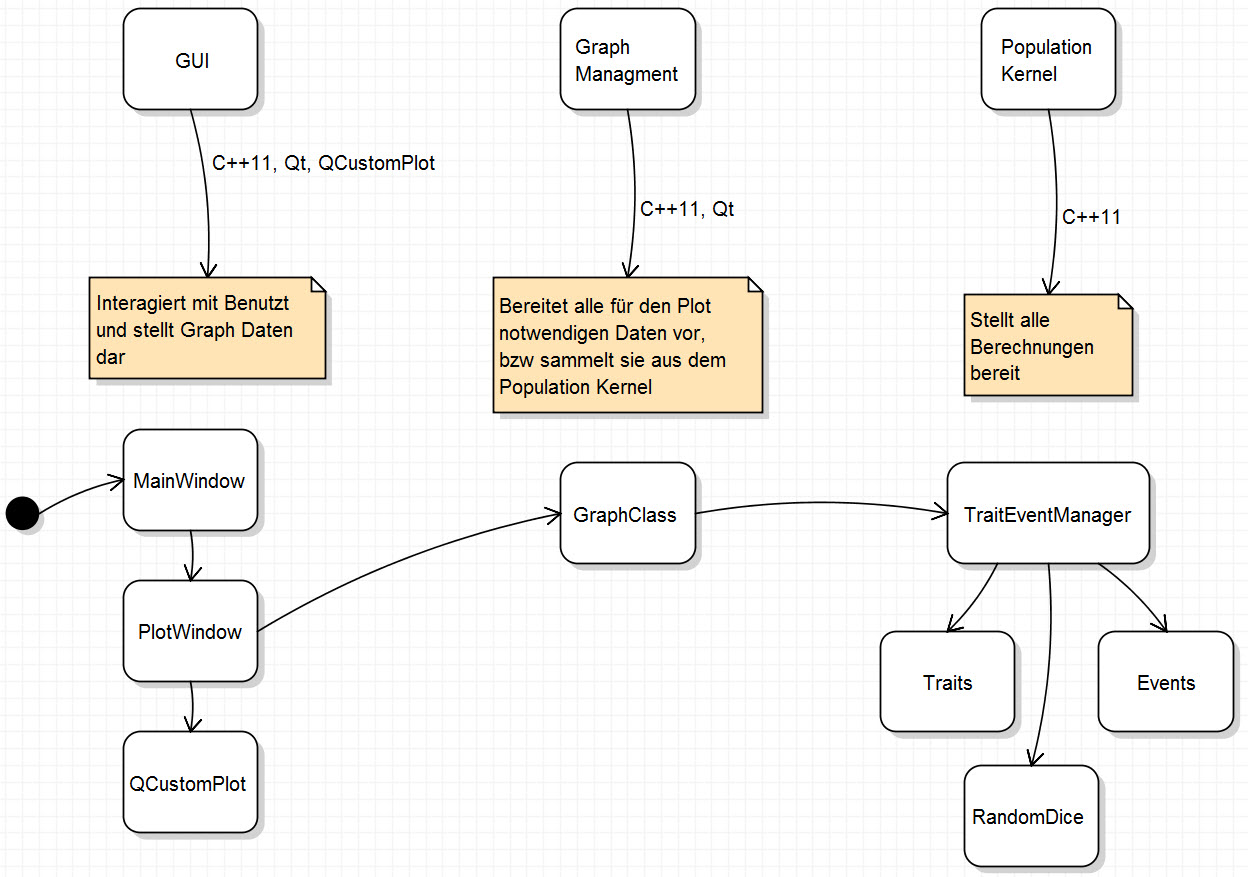
\includegraphics[width=0.7\linewidth]{./Pictures/Bild_Module}
		\caption[Module]{Arbeitsmodule und Klassenabhängigkeiten}
		\label{Module und Klassen}
	\end{figure}
	Innerhalb der Arbeitsschritte sollte dabei genau die selbe Regel der Unabhängigkeit gelten wie bei den Modulen.
	
	\subsection{Layout}
	\begin{itemize}
		\item Die Bedienung des Programms sollte das lesen und Anzeigen der Merkmals-Parameter bereitstellen. Da es viele Parameter gibt und die Anzahl der Parameter quadratisch mit der Anzahl der betrachteten Merkmale steigt, bietet sich das Lesen aus zuvor beschriebenen Dateien an.
		\begin{figure}[H]
			\centering
			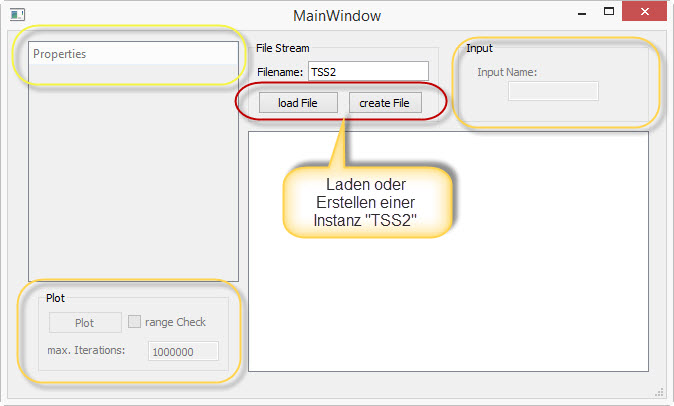
\includegraphics[width=0.7\linewidth]{./Pictures/MainWindow_Start}
			\caption[Startwindow]{MainWindow nach dem Start}
			\label{MainWindow_Start}
		\end{figure}

		Zur Darstellung der gelesenen Parameter habe ich ein Baumstruktur gewählt.
		\begin{figure}[H]
			\centering
			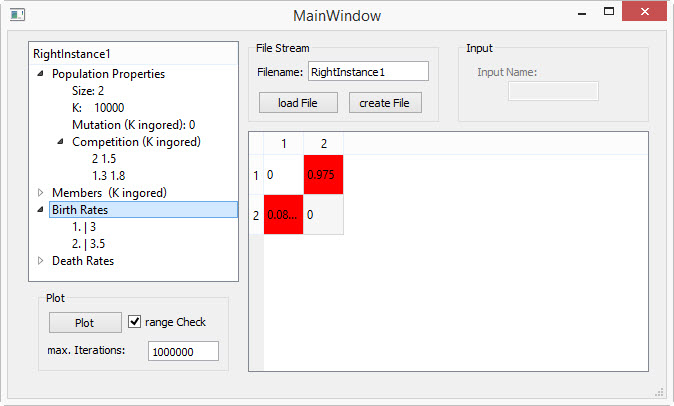
\includegraphics[width=0.7\linewidth]{./Pictures/MainWindow_ParameterBaum}
			\caption[MainWindow_Parameter]{MainWindow mit geladenen Parametern}
			\label{Baumstruktur}
		\end{figure}
		\item Die letzte Herausforderung bestand darin eine Instanz durch das Programm geleitet erstellen zu können. Während diese Aufgabe bei einer Konsolenanwendung (bekannt aus den klassischen c Programmen) denkbar einfach mit "{}printf"{} und "{}scanf"{} erledigt werden konnte, sollte bei einem GUI eine Lösung her die Inputkonflikte verhindert und das Einlesen der Daten denkbar einfach macht. Dafür war es sinnvoll "{}Enter"{} als Bestätigung abzufangen und sicherzustellen dass der Curser nur innerhalb des gewünschten Feldes bleibt.
		\begin{figure}[H]
			\centering
			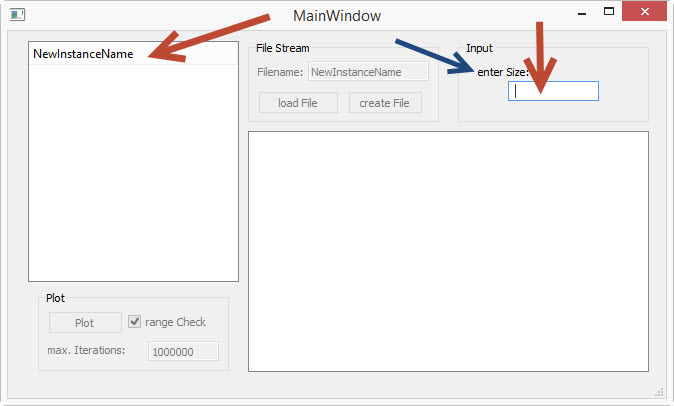
\includegraphics[width=0.7\linewidth]{./Pictures/MainWindow_createFile}
			\caption[erstelle Datei]{Nach Klick auf "{}create File"{} werden die neuen Parameter einzeln abgefragt}
			\label{fig:MainWindow_createFile}
		\end{figure}
		\begin{figure}[H]
			\centering
			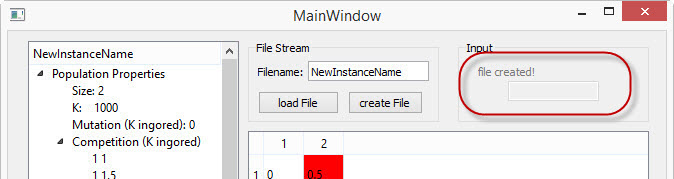
\includegraphics[width=0.7\linewidth]{./Pictures/MainWindow_FileCreated}
			\caption[Datei erstellt]{Nach Eingabe des letzten Parameters}
			\label{fig:MainWindow_FileCreated}
		\end{figure}
	\end{itemize}
	Was die Darstellung der Graphen angeht, hat sich ein einfaches Bild des fertigen Plots durchgesetzt, wobei das Zoomen und ziehen des Bildes notwendige Elemente zur Untersuchung des Graphen sind. Zusätzlich ist es notwendig viele Bilder vergleichen zu können. Hierfür wurde das Abspeichern des Bildes gewünscht.\\
	Die Simulation wird gestartet nachdem man auf den "{}Plot"{} Button drückt. Dabei wird ein neues Fenster geöffnet.
	\begin{figure}[H]
		\centering
		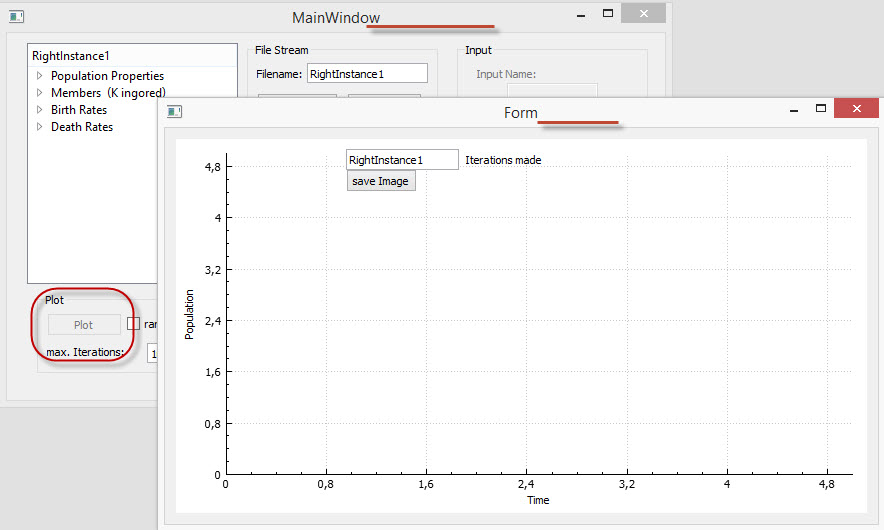
\includegraphics[width=0.7\linewidth]{./Pictures/PlotWindow_start}
		\caption[PlotWindow_start]{Start des PlotWindow}
		\label{PlotWindow_start}
	\end{figure}
	Sobald der Plot Button gedrückt wurde und das Fenster angezeigt wird, arbeitet die Simulation bereits im Hintergrund in einem eigenen Thread. Dort werden alle notwendigen Iterationen bzw. Sprünge der Population durchgeführt ohne den Hauptthread damit zu belasten.\\ Während dieser Arbeiterthread aktiv arbeitet wird der "{}Plot"{} Button ausgegraut um mehrfaches Auslösen zu vermeiden und um anzuzeigen dass die Rechnung im Gange ist.\\
	Der Arbeiterthread gewährleistet nicht nur eine flüssige Interaktion mit dem Programm, sondern verhindert auch effektiv dass das Betriebssystem denkt das Programm wäre Abgestürzt oder würde nicht mehr ordnungsgemäß funktionieren. Das würde sonst folgendes evtl. bekannte Bild hervorrufen:
	\begin{figure}[H]
		\centering
		
\includegraphics[width=0.7\linewidth]{./Pictures/KeineRueckmeldung}
		\caption[Keine Rueckmeldung]{Hauptthread wurde überlastet}
		\label{Keine Rueckmeldung}
	\end{figure}
	Wenn die Simulation  einen gewünschten Zustand erreicht hat, oder die maximale Anzahl an gewünschten Iterationen absolviert hat, werden anschließend maximal 10mio Punkte auf dem Koordinatensystem zu Graphen verbunden. Das kann so aussehen:
	\begin{figure}[H]
		\centering
		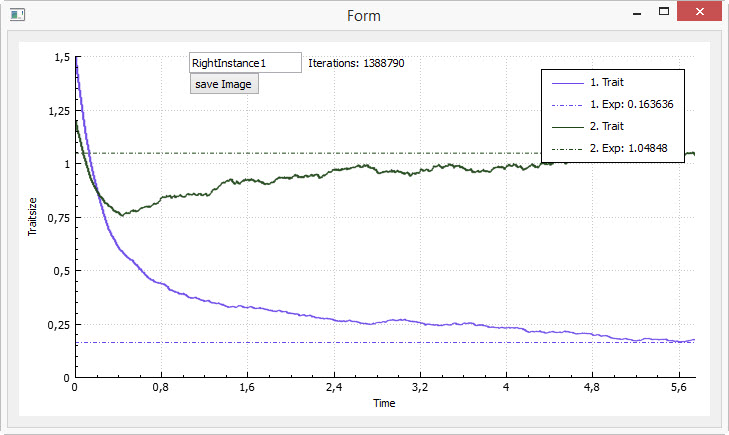
\includegraphics[width=0.7\linewidth]{./Pictures/PlotWindow_smallBPDL}
		\caption[PlotWindow]{PlotWindow mit Dimorpher Population}
		\label{PlotWindow}
	\end{figure}

\clearpage
\section{Verhaltenstest - Korrektheit der Implementation}
(Korrektheit des Algorithmus nicht notwendig bzw möglich)
Ein ganz besonders interessantes Thema ist die Korrektheit der Implementation. Diese ist generell mit steigender Komplexität schwerer zu prüfen (besonders bei Zufallsbedingten Simulationen).\\
Daher habe ich das Prinzip der "{}Testgetriebene Entwicklung"{}  (Test Driven Develeopment) verwendet.\\
Dabei werden Funktionen des Programms unter vorher festgelegten Bedingungen laufen gelassen und mit einem erwarteten Verhalten verglichen. Das Ergebnis ist eine Ausgabe für Erfolg oder Misserfolg des Tests. Folgend ein Beispiel für eine Implementation eines einfachen Tests der prüft ob alle Parameter korrekt aus der Datei in die Objekte geschrieben werden.
\begin{figure}[H]
	\centering
	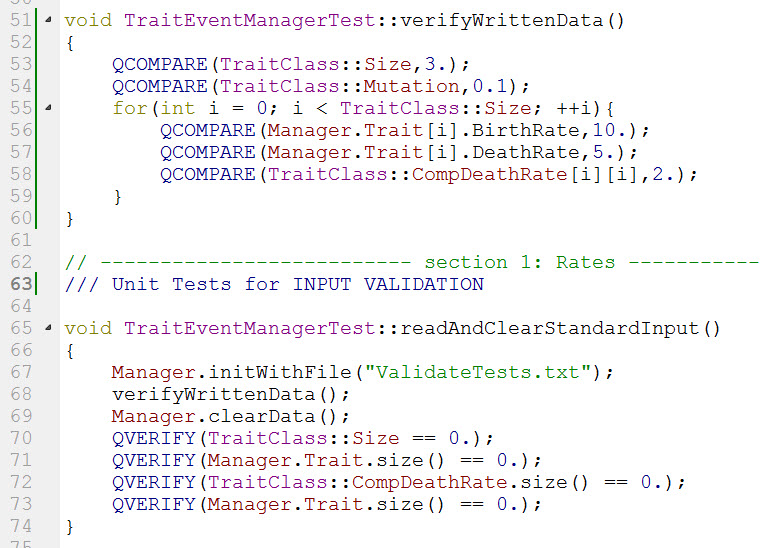
\includegraphics[width=0.7\linewidth]{./Pictures/UnitTest}
	\caption[UnitTest]{UnitTest versichert korrektes lesen von Parametern aus Datei}
	\label{Unit Test}
\end{figure}
Anschließend ein Beispiel für einen Durchlauf der Testfunktionen:
\begin{figure}[H]
	\centering
	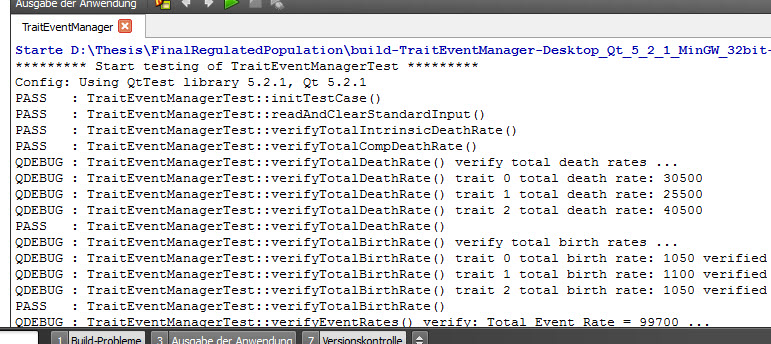
\includegraphics[width=0.7\linewidth]{./Pictures/TestResult_start}
	\caption[Test Resultat einer Test Datei]{Ergebnisse einiger Tests}
	\label{Test Results}
\end{figure}
Die Testfunktionen zeigen auch dass eine komplexe Verwendung der Simulationen über die graphische Darstellung hinaus einfach realisierbar ist.

	\subsection{Unit Tests der Algorithmusmodule}

\clearpage
\section{TSS Prozesse}
\noindent\rule{\textwidth}{2pt}
\begin{center}
	$ <<< \quad \downarrow $ Reserviert $ \downarrow \quad >>> $
\end{center}
\begin{center}
	\textbf{Frage:} Warum soll $ \mu_K $ in dem Bereich 
	\[ \left( \frac{1}{e^{VK}} << \mu_K << \frac{1}{K log(K)} \right), \] 
	gew"ahlt werden?\\
\end{center}

\textbf{Antwort:} Dank Freidlin and Wenzell \cite{freidlin2012random} erwarten wir dass unsere dominante Spezies $ exp(cK) $ Zeiteinheiten im Equilibrium bleibt. Schlie"slich k"onnen wir so kontrollieren wie lange uns eine dominante Spezies die f"ur eine mutative Geburt in Frage kommt erhalten bleibt. Und dadurch dass eine unsere Mutationen exponentiell verteilt sind ben"otigt man ein eine Rate $ \mu_K >> \frac{1}{e^{cK}} $ um eine Zeit von $ exp(cK) $ nicht zu "uberschreiten, was die erste Schranke rechtfertigt.\\
Um die zweite Schranke zu Rechtfertigen betrachten wir nun die Zeit die ein Mutant braucht um ein dominantes Merkmal aussterben zu lassen. Das wird uns die M"oglichkeit geben einer neuen Mutation so viel Zeit zu lassen bis das derzeit benachteiligte Merkmal ausgestorben ist.\\
Angenommen es ereignet sich eine Mutation und der Mutant $ x $ ist fitter ($ f(x,y) > 0 $), so wird es mit positiver Wahrscheinlichkeit eine Invasion ausl"osen. Wenn man Branching Prozesse mit dem Lotka-Volterra System vergleicht, kommt man darauf dass die ben"otigte Zeit zum Verdr"angen und Aussterben des urspr"unglich dominanten Merkmals von der Ordnung $ \log(K) $ ist.
Diese Invasion wird eine Zeit von der Ordnung $ \log(K) $ ben"otigen. Das l"asst sich folgern indem man Branching Prozesse mit 

\begin{center}
	$ <<< \quad \uparrow $ Reserviert $ \uparrow \quad >>> $
\end{center}
\noindent\rule{\textwidth}{2pt}

Bei TSS Prozessen beobachten wir wie sich Merkmale gegeneinander durchsetzten und sich verdrängen. (Tafelbild)\\
Genau wie bei der LPA-Normalisierung ergeben sich TSS-Prozesse(Trait Substitution Sequence) als Grenzprozesse von BPDL-Prozessen. Zu der LPA-Normalisierung sollten jedoch mit größer werdendem K die Mutationen seltener werden ($ \frac{1}{e^{VK}} << \mu_K << \frac{1}{K log(K)} $) , also die Mutationswahrscheinlichkeit gegen 0 streben. Skaliert man nun noch zusätzlich die Zeit, so führt dies dazu, dass die Zeit, die ein Merkmal benötigt, um sich gegenüber einem anderen durchzusetzen und dieses zu verdrängen, infinitesimal klein wird. Somit simulieren die TSS-Prozesse eine Population, die zu jedem Zeitpunkt monomorph ist und sich im entsprechenden (für $ K < \infty $ angepassten) Gleichgewicht befindet.\\
Spätestens jetzt wird die Fitness-Funktion interessant:
\[ f(x,y) = b(x) - d(x) - c(x,y)\bar{n}_y \]
Diese Fitness-Funktion gibt an, wie gut sich ein Merkmal gegenüber einem anderen durchsetzen kann. Sie ist die asymptotische Wachstumsrate von y, wenn x sich im Gleichgewichtszustand $ \bar{n}_x $ befindet und nur wenige Individuen von Typ y in der Population vorhanden sind. In der Simulation sieht man die Fitness der Merkmale zueinander in einer Matrix nach dem Laden der Parameter.
\begin{figure}[H]
	\centering
	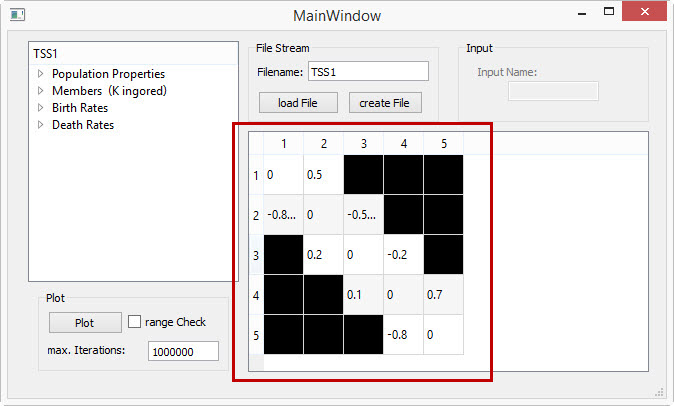
\includegraphics[width=0.7\linewidth]{./Pictures/MainWindow_BandMatrix}
	\caption[Fitness Matrix]{Fitness Bandmatrix}
	\label{MainWindow mit Fitness Bandmatrix}
\end{figure}
Mit der Fitness kann man eine Konvergenz der Wahrscheinlichkeit für das überleben einer Mutation vorhersagen:
\[ \frac{\left[ f(y,x)\right]_+ }{b(y)} \]
Da diese Wahrscheinlichkeit gerne bereits beim einlesen der Parameter angezeigt werden will, habe ich vor sie als farblich ansteigenden Akzent den Elementen der Zelle hinzuzufügen. Bisher wird in der Matrix etwas grün oder rot markiert. Rot falls eine Koexistenz vorliegt und grün wenn die Wahrscheinlichkeit für Dominanz des Mutanten über 50\% liegt.
\begin{figure}[H]
	\centering
	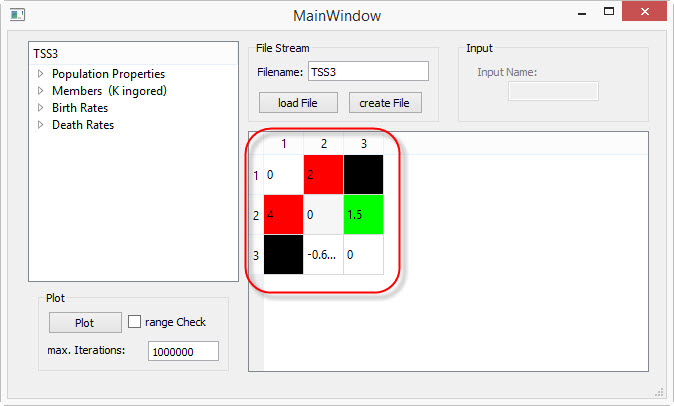
\includegraphics[width=0.7\linewidth]{./Pictures/MainWindow_red_green_loaded}
	\caption[MainWindow_redGreenFitness]{Fitness Matrix mit roten und gruenen akzenten}
	\label{fig:MainWindow_red_green_loaded}
\end{figure}
Wenn der einfache BPDL Simulator für die Simulation dieses Prozesses verwendet werden würde, würde durch die seltenen Mutationen

	\subsection{Optimierung}
	Hier stelle ich die lineare Interpolation als eine Optimierung vor die "Ubersichtlichkeit, Analyse und Laufzeit deutlich verbessert. Dann beschreibe ich anhand von Bildern wie gut man Mutationen und deren Auswirkungen verfolgen kann und wie ich gepr"uft habe ob auch hier alles Korrekt l"auft.\\
	Schlie"slich erkl"are ich wie ich die Mutationszeitpunkte ermittelt habe.
	
	\subsection{Aufwand}
	H"angt nicht mehr nur von K ab...
	
	\subsection{Algorithmus}
\clearpage
\section{Ausblick}

\begin{itemize}
	\item Weiteres Abbruchkriterium = Zeit : sehr einfach zu implementieren.
\end{itemize}

\clearpage
\bibliography{science1}

\clearpage

\section{Beweise}


\section{Fragen}
\begin{itemize}
	\item Normalisierung, Gleichgewicht und mono/dimorphe F"alle als einzelne Kapitel?
	\item Soll ich monomorphe BPDL Prozesse einf"uhren? Schlie"slich kann ich damit das fast sicheres Aussterben 
	\item Beweis der LPA-Normalisierung per Differentialgleichungen?
\end{itemize}

\section{Wozu hat es nicht mehr gereicht?}
Instanzbrowser oder Dateisuche.\\
einfaches Bearbeiten erstellter Instanzen.\\

\end{document}